\chapter{Differentiation}
We consider $f:[a,b]\to \R$.

\begin{definition*}
	For $f: [a,b]\to \R$ and $x \in [a,b]$, let $f'(x)=\lim_{t\to x}{\frac{f(t)-f(x)}{t-x}}$ if limit exists.
	Equivalently, $f(t)=f(x)+(t-x)[f'(x)+u(x,t)]$ with $\lim_{t\to x}{u(x,t)}=0$.
\end{definition*}

\begin{example}
	\begin{enumerate}[label=(\alph*)]
		\item $f(x)=c \; \text{ for all } x \implies f'(x)=\lim_{t\to x}{\frac{c-c}{t-x}}=0$.
		\item $f(x)=x\; \text{ for all }x\implies f'(x)=\lim_{t\to x}{\frac{t-x}{t-x}}$
		\item $f(x)=e^{x}:=\sum_{n=0}^{\infty}{\frac{x^{n}}{n!}}$.
		      Write $t=x+h$, so $t\to x \Leftrightarrow h\to 0$.
		      $\frac{e^{x+h}-e^{x}}{(x+h)-x}=e^{x}\frac{e^{h}-1}{h}=e^{x}\frac{e^{h}-1}{h}+e^{x}-e^{x}=e^{x}+e^{x}\frac{e^{h}-1-h}{h}$.
		      Let $u(h)=\frac{e^{h}-1-h}{h}$. Then $u(h)=\frac{1}{h}\sum_{n=2}^{\infty}{\frac{h^{n}}{n!}}$, so $|u(h)|=|\frac{1}{h}\sum_{n=2}^{\infty}{\frac{h^{n}}{n!}}|\le |h| \sum_{n=2}^{\infty}{\frac{1}{n!}}=(e-2)|h|$ (note for $n\ge 2, |h^{n-1}|\le |h|$ if $|h|\le 1$). Hence, $u(h)\to \infty$ as $h\to 0$ and therefore $f'(x)=e^{x}$.
		      \begin{remark}
			      $e^{x}:=\sum_{n=0}^{\infty}{\frac{x^{n}}{n!}}$ is well defined.
			      $e^{1}=\sum_{n=0}^{\infty}{\frac{1}{n!}}=e$. Regarding it as a power series, its radius of convergence is $R=\infty$. Also, $e^{x+y}=e^{x}e^{y}$ using definition 3.48 of product series (Rudin's p.178-180).
		      \end{remark}
		      \begin{note}
			      $f'(x)$: Lagrange's notation, $\frac{df}{dx}$: Leibnitz notation
		      \end{note}
	\end{enumerate}
\end{example}

\begin{thm}[2]
	Suppose $f:[a,b]\to \R$ and $f'(x)$ exists. Then $f$ is continuous at $x$.
	\begin{proof}
		The existence of $f'(x) \Leftrightarrow f(t)=f(x)+(t-x)[f'(x)+u(x,t)]$ with $\lim_{t\to x}{u(x,t)}=0$. Let $t\to x$. $\lim_{t\to x}{f(x)+(t-x)[f'(x)+u(x,t)]}=f(x)+0[f'(x)+0]=f(x)$, so $\lim_{t\to x}{f(t)}=f(x)$; i.e., $f$ is continuous at $x$.
	\end{proof}
	\begin{remark}
		The converse is false; e.g., $f(x)=|x|$ is continuous for all $x$, but $f'(0)$ does not exist.
	\end{remark}
\end{thm}

\begin{thm}[3]
	If $f:[a,b]\to \R$ and $g:[a,b]\to \R$ are both differentiable at $x$ then so are $f+g,fg,\frac{f}{g}(\text{ if } g(x)\neq 0)$, and $(f+g)'(x)=f'(x)+g'(x),(fg)'(x)=f'(x)g(x)+f(x)g'(x),(\frac{f}{g})'(x)=\frac{f'(x)g(x)-g'(x)f(x)}{g(x)^2}$. \end{thm}
\begin{proof}[Only the quotient rule]
	$h(t)-h(x)=\frac{f(t)}{g(t)}-\frac{f(x)}{g(x)}=\frac{1}{g(t)g(x)}[(f(t)g(x)-f(x)g(x))-(f(x)g(t)-f(x)g(x))]$.\\
	Then $\frac{h(t)-h(x)}{t-x}=\frac{1}{g(t)g(x)}\left[ \frac{f(t)-f(x)}{t-x}g(x)-f(x)\frac{g(t)-g(x)}{t-x} \right]$.
	Let $t\to x$. $h'(x)=\frac{1}{g(x)^2}\left[ f'(x)g(x)-f(x)g'(x) \right] ]$.
\end{proof}
\begin{remark}
	By induction, $(f_1\cdots f_n)'=f_1'f_2\cdots f_n+f_1 f_2'f_3\cdots f_n+ \cdot f_1 f_2 \cdots f_n'$.
	\begin{example}
		For $n=2,3$,
		$\dfrac{d}{dx}x^{n}=nx^{n-1}$ and we know this already for $n=0,1$.
		For $n=-1,-2$, let $m=-n>0$. Then $\dfrac{d}{dx}x^{n}=\dfrac{d}{dx}\dfrac{1}{x^{m}}=\dfrac{(\dfrac{d}{dx}1)x^{m}-(\dfrac{d}{dx}x^{m})1}{(x^{m})^2}=\dfrac{0x^{m}-mx^{m-1}1}{x^{2m}}=-mx^{m-1}=nx^{n-1}$. Hence, $\forall_{n \in \Z}: \dfrac{d}{dx}^{n}=nx^{n-1}$.
	\end{example}
\end{remark}

\begin{thm}[5][Chain Rule]
	Suppose $f:[a,b]\to \R$, $f'(x)$ exists for some $x \in [a,b], f([a,b]) \subset I$, where $I$ is some interval in $\R$. Suppose $g: I\to \R$ and $g'(f(x))$ exists. Then $g \circ f$ is differentiable at $x$ and $(g\circ f)(x)'=g'(f(x))f'(x)$
	\begin{proof}
		Let $h(t)=(g\circ f)(t)=g(f(t))$ for $t \in [a,b]$. Fix $x \in [a,b]$ where $f'(x)$ exists. We know:
		\begin{enumerate}
			\item $f(t)-f(x)=(t-x)[f'(x)+u(t)]$ with $\lim_{t\to x}{u(t)}=0$.
			\item With $y=f(x)$, $g(s)-g(y)=(s-y)(g'(y)+v(s))$ with $\lim_{s\to y}{v(s)}=0$
		\end{enumerate}
		As $\dfrac{h(t)-h(x)}{t-x}=\dfrac{g(f(t))-g(f(x))}{t-x}$. By (2), $\dfrac{g(f(t))-g(f(x))}{t-x}[g'f(x)+v(f(t))]$.
		Let $t\to x$. Then $\text{ RHS } \to f'(x)[g'(f(x))+0]$ since $f(t)\to f(x)$ by continuity of $f$ at $x$. Therefore, $h'(x)=f'(x)g'(f(x))$.
	\end{proof}
	\begin{note}
		Suppose you produce $f(t)$ meters of wire by time $t$; i.e., rate of wire production is $f'(t) \;m/x$. Also suppose you get $\$\; g(l)$ for $l$ meters of wire; rate of profit is $g'(l) \;\$/m$. Then the rate of earning by time $t$ is $g'(f(t))f'(t) \;\$/m$.
	\end{note}
\end{thm}

\begin{example}
	\begin{enumerate}
		\item $\dfrac{d}{dx}e^{x^2}=2xe^{x^{2}}$
		\item $f(x)=\begin{cases}
				      x \sin{\dfrac{1}{x}} & \text{ if } x\neq 0 \\
				      0                    & \text{ if } x=0
			      \end{cases}$
		      \begin{remark}
			      \begin{enumerate}
				      \item
				            $f$ is continuous on $\R$, including at $x=0$.
				            \begin{proof}
					            $|f(x)|\le |x|$, so by the Squeeze theorem, $\lim_{x\to 0}{f(x)}=0=f(0)$.
				            \end{proof}
				      \item $f$ is differentiable on $x\neq 0$, but not differentiable at $x=0$.
				            For $x\neq 0$, $f'(x)=\sin{\dfrac{1}{x}}+x(\cos{\dfrac{1}{x}})(\dfrac{-1}{x^2})=\sin{\dfrac{1}{x}}-\dfrac{1}{x}\cos{\dfrac{1}{x}}$.
				            For $x=0$, $\dfrac{f(t)-f(0)}{t-0}=\dfrac{t \sin{\dfrac{1}{t}}}{t}=\sin{\dfrac{1}{t}}$, which does not converge. Therefore, $f$ not differentiable at $x=0$.
			      \end{enumerate}
		      \end{remark}
		\item Let $f(x)= \begin{cases}
				      x^2 \sin{\dfrac{1}{x}} & \text{ if } x\neq 0 \\
				      0                      & x=0
			      \end{cases}$.
		      \begin{enumerate}
			      \item
			            $f$ is continuous in $\R$ including at $x=0$ ($\because |f(x)|\le |x^2|$).
			      \item $f$ is differentiable in $\R$ including at $x=0$.
			            \begin{proof}
				            For $x\neq 0$, $f'(x)=2x \sin{\dfrac{1}{x}}+x^2(\cos{\dfrac{1}{x}})(\dfrac{-1}{x^2})=2x \sin{\dfrac{1}{x}}-\cos{\dfrac{1}{x}}$.
				            For $x=0$, $\dfrac{f(t)-f(0)}{t-0}= \dfrac{t^2 \sin{\dfrac{1}{t}}}{t}=t \sin{\dfrac{1}{t}}\to 0$ as $t\to 0$. Hence, $f'(0)=0$.
				            HOWEVER! $f'$ is not continuous at $x=0$, because $\lim_{x\to 0}{f'(x)}$ does not exist.
			            \end{proof}
		      \end{enumerate}
	\end{enumerate}
\end{example}

\begin{definition}
	\label{def:5.7}
	Let $X$ be a metric space, $f:X\to \R$. $f$ has a \textit{local} max at $x \in X$ if $\exists_{\delta > 0} \text{ s.t. } f(y)\ge f(x)$ for all $y \in N_{\delta}(x)$.
\end{definition}
\begin{thm}[8]
	Let $f:[a,b]\to \R$. If $f$ has a local min or a local max at $x \in (a,b)$ and if $f'(x)$ exists, then $f'(x)=0$.
	\begin{proof}[local min]
		Suppose $f$ has a local min at $x$ and $f'(x)$ exists. Choose $\delta>0$ s.t. $N_{\delta}(x) \subset (a,b)$ and $f(t)\ge f(x)$ if $t \in (x-\delta,x+\delta)$.
		For $x<t<x+\delta,$ $\dfrac{f(t)-f(x)}{t-x}\ge 0 (\because f(t)\ge f(x),t>x)$, so $f'(x)\ge 0$.
		For $x-\delta<t<x$, $\dfrac{f(t)-f(x)}{t-x}\le 0 (\because f(t)-f(x)\ge 0, t<x)$, so $f'(x) \le 0$.
		Hence, $f'(x)=0$.
	\end{proof}


	\begin{remark}
		Note that the hypothesis of the theorem requires \textit{open} interval and existence $f'(x)$. If these conditions are not met, then $f'(x)=0$ doesn't have to be the case.
		\begin{example}
			\begin{enumerate}
				\item $f(x)=|x|$ has a local min at $x=0$ but $f'(0)$ does not exist.
				\item $f:[0,1]\to \R$ defined by $f(x)=x$ has a local max at $x=1$ and local min at $x=0$, but $f'(0)=f'(1)=1$.
			\end{enumerate}
		\end{example}
	\end{remark}
\end{thm}

\begin{thm}[10][Mean-Value Theorem]
	If $f:[a,b]\to \R$ is continuous and differentiable on $(a,b)$, then $\exists_{x \in (a,b)} \text{ s.t. } f(b)-f(a)=f'(x)(b-a)$.
	\begin{proof}
		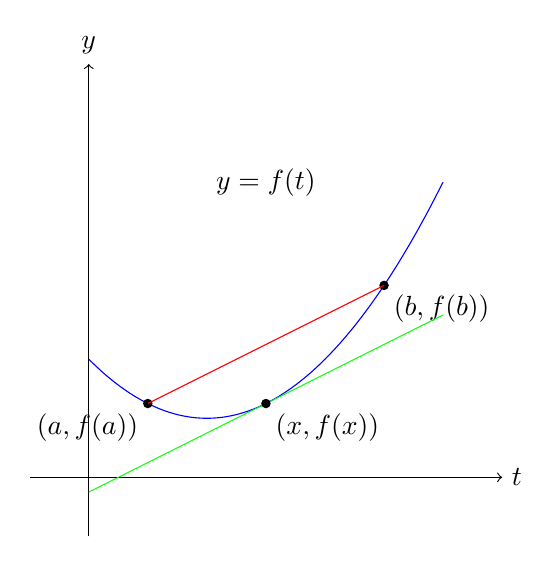
\begin{tikzpicture}[scale=1.5]
			% Define the function f(t)
			\def\fa{0.5}
			\def\fb{2.5}
			\def\fc{1.5}
			\def\fd{1.5}
			\def\fe{1.5}
			\def\ff{1.5}
			% Draw the axes
			\draw[->] (-0.5,0) -- (3.5,0) node[right] {$t$};
			\draw[->] (0,-0.5) -- (0,3.5) node[above] {$y$};
			% Draw the function y=f(t)
			\draw[domain=0:3,smooth,variable=\t,blue] plot ({\t},{0.5*\t*\t - \t + 1});
			% Points (a, f(a)) and (b, f(b))
			\filldraw[black] (\fa,{0.5*\fa*\fa - \fa + 1}) circle (1pt) node[below left] {$(a, f(a))$};
			\filldraw[black] (\fb,{0.5*\fb*\fb - \fb + 1}) circle (1pt) node[below right] {$(b, f(b))$};
			% Draw the secant line from (a, f(a)) to (b, f(b))
			\draw[red] (\fa,{0.5*\fa*\fa - \fa + 1}) -- (\fb,{0.5*\fb*\fb - \fb + 1});
			% Calculate the slope of the secant line
			\pgfmathsetmacro{\m}{(0.5*\fb*\fb - \fb + 1 - (0.5*\fa*\fa - \fa + 1))/(\fb - \fa)}
			% Draw the tangent line at some point c
			\pgfmathsetmacro{\fc}{1.5}
			\pgfmathsetmacro{\fcx}{\fc}
			\pgfmathsetmacro{\fcy}{0.5*\fc*\fc - \fc + 1}
			\draw[domain=0:3,smooth,variable=\t,green] plot ({\t},{\m*(\t-\fcx) + \fcy});
			% Point (c, f(c))
			\filldraw[black] (\fc,{0.5*\fc*\fc - \fc + 1}) circle (1pt) node[below right] {$(x, f(x))$};
			% Labels
			\node at (1.5,2.5) {$y=f(t)$};
			\node at (2.5,1.5) [red] {};
			\node at (1,2) [green] {};
		\end{tikzpicture}
		Let $L: y=f(a)+m(t-a)$, where $m=\dfrac{y-f(a)}{t-a}=\dfrac{f(b)-f(a)}{b-a}$.
		Subtract $L$ from the curve $y=f(t)$. Let $h(t)=f(t)-[f(a)+m(t-a)]$.
		Then $h(a)=h(b)=0$. $h'(t)=f'(t)-m=f'(t)-\dfrac{f(b)-f(a)}{b-a}$.
		Therefore, it suffices to find $x$ s.t. $h'(x)=0$.
		$h$ is continuous and $[a,b]$ is compact, so $h([a,b])$ is also compact.
		Hence, $h$ attains its global max($=\sup\{h([a,b])\}$) and global min($=\inf\{h([a,b])\}$) on $[a,b]$.
		If $h(t)=0$ for all $t \in [a,b]$ then $h'(t)=0$ for all $t \in [a,b]$ so any $x \in (a,b)$ will do.
		Otherwise, $h$ attains its global max or global min at some $x \in (a,b)$. By Theorem~\ref{thm:5.8}, $h'(x)=0$.
	\end{proof}
\end{thm}

\begin{thm}[11]
	If $f$ is differentiable on $(a,b)$ then
	\begin{enumerate}
		\item  $f'(x)\ge 0$ for all $x \in (a,b)$ implies $f$ is monotone increasing.
		\item  $f'(x)\le 0$ for all $x \in (a,b)$ implies $f$ is monotone decreasing.
		\item  $f'(x)= 0$ for all $x \in (a,b)$ implies $f$ is constant.
	\end{enumerate}
	\begin{proof}[(a) only]
		Suppose $f'(x)\ge 0$ for all $x \in (a,b)$.
		For $a<x_1<x_2<b$, $\exists_{x \in (x_1,x_2)} \text{ s.t. } f(x_2)-f(x_1)=f'(x)(x_2-x_1)$ by Theorem~\ref{thm:5.10}.
		As $f'(x)\ge 0, x_2\ge x_1$, $f(x_2)-f(x_1)\ge 0$.
	\end{proof}
\end{thm}

\begin{definition}
	$f^{(0)}=f, f^{(1)}=f', f^{(2)}=f'', f^{(3)}=f'''$ and so on.
\end{definition}

\begin{thm}[15][Taylor's Theorem]
	Suppose $f:[a,b]\to \R$, $n \in \N$, and $f^{(n+1)}(x)$ exists for all $x \in (a,b)$.
	Let $x, x_0 \in [a,b]$. Then $\exists_{c \in (x, x_0)} \text{ s.t. }$
	\[f(x)=\underbrace{\sum_{k=0}^{n}{\dfrac{f^{(k)}(x_0)}{k!}(x-x_0)^{k}}}_{P_n(x),\text{$n^{\text{th}}$ Taylor polynomial of $f$ at $x_0$}}+\underbrace{\dfrac{f^{(n+1)}(c)}{(n+1)!}(x-x_0)^{n+1}}_{\text{Taylor Remainder}}.\]
	\begin{proof}
		If $n=0$, the mean-value theorem guarantees existence of $c$.
		For general $n$, $A \in \R$ by $R_n(x)=f(x)-P_n(x)=\dfrac{A}{(n+1)!}(x-x_0)^{n+1}$, where $A$ depends on $f,n,x,x_0$.
		Claim: $A=f^{(n+1)}(c)$ for some $c$ between $x$ and $x_0$.\\
		Define $g(t)=f(t)-P_{n}(t)-\dfrac{A}{(n+1)!}(t-x_0)^{n+1}$ for $t \in [a,b]$. Then $g(x_0)=0$.
		$g(x)=f(x)-P_{n}(x)-\dfrac{A}{(n+1)!}(x-x_0)^{n+1}=0$ by the definition of $A$.
		Also for $j=1,\ldots ,n$, then $P_{n}^{(j)}(x_0)=f^{(j)}(x_0)$, $\dfrac{\mathrm{d}^{j}}{\mathrm{d}x^{j}}(x-x_0)^{n+1} \mid_{x=x_0}=0$.
		Hence, $g^{(j)}(x_0)=f^{(j)}(x_0)-P_{n}^{(j)}(x_0)-0=0$.
		$g^{(n+1)}(t)=f^{(n+1)}(t)-0-A$.
		We need to find $c$ s.t. $g^{(n+1)}(c)=0$.
		$g(x)=g(x_0)=0 \implies \exists_{c_1 \in (\min\{x_0,x\},\max\{x_0,x\})} \text{ s.t. } g'(c_1)=0$.\\
		$g'(x_0)=g'(c_1)=0 \implies \exists_{c_2 \in (\min\{x_0,x,c_1\},\max\{x_0,x,c_1\})} \text{ s.t. } g''(c_2)=0$.\\
		$\vdots$\\
		Finally, $\exists_{c_{n+1}=c} \text{ s.t. } g^{n+1}(c)=0$ and hence $f^{(n+1)}(c)=A$.
	\end{proof}
\end{thm}
\begin{example}
	(not in Rudin)
	Does $\sum_{n=1}^{\infty}{\left( \sqrt{1+\dfrac{1}{n^2}}-1 \right)}$ converge or diverge?
	Method 1:
	\[
		\sqrt[]{1+\dfrac{1}{n^2}}-1=\dfrac{\left(\sqrt[]{1+\dfrac{1}{n^2}}-1\right)\left(\sqrt[]{1+\dfrac{1}{n^2}}+1\right)}{\sqrt[]{1+\dfrac{1}{n^2}}+1}
		=\dfrac{1+\dfrac{1}{n^2}-1}{\sqrt[]{1+\dfrac{1}{n^2}}+1}=\dfrac{1}{n^2}\dfrac{1}{\sqrt{1+\dfrac{1}{n^2}}+1}\le \dfrac{1}{n^2}
		,\] so the series converges by the comparison test since $\sum{\dfrac{1}{n^2}}$ converges.\\
	Method 2: Using Taylor's theorem. Let $f(x)=\sqrt[]{1+x}=(1+x)^{1/2}$. Then
	\begin{align*}
		f'(x)  & =\dfrac{1}{2}(1+x)^{-1/2}                                            \\
		f''(x) & =\dfrac{1}{2}(-\dfrac{1}{2})(1+x)^{-3/2}  =-\dfrac{1}{4}(1+x)^{-3/2} \\
		f(x)   & =P_1(x)+R_1(x)                                                       \\
		       & =f(0)+\dfrac{f'(0)}{1!}(x-0)^{1}+\dfrac{f''(c)(x-0)^{2}}{2!}         \\
		       & =1+\dfrac{1}{2}x+R_1(x)
		.\end{align*}
	$|R_1(x)|\le (\dfrac{1}{2}\cdot \dfrac{1}{2}\cdot 1)\dfrac{1}{2!}x^{2}=\dfrac{1}{8}x^2$ for $x \in [0,1]$.
	Therefore, $\sqrt[]{1+\dfrac{1}{n^2}}-1=f(\dfrac{1}{n^2})-1=\dfrac{1}{2}(\dfrac{1}{n^2})+R_1(\dfrac{1}{n^2})\le \dfrac{1}{2n^2}+\dfrac{1}{8}\dfrac{1}{n^{4}}$.
	Since $\sum{\left(\dfrac{1}{2n^2} +\dfrac{1}{8n^{4}}\right)}$ converges, $\sum{\left(\sqrt[]{ 1+\dfrac{1}{n^2}}-1 \right)}$  converges by comparison test.
\end{example}

\begin{example}
	Let $f(x)=\sin{x}, x_0=0$.
	\begin{description}
		\item[Taylor series for $f(x)$.]
		      $f'(x)=\cos{x}, f''(x)=-\sin{x}, f'''(x)=-\cos{x},\ldots $, so
		      $f^{(k)}(x)=\begin{cases}
				      (-1)^{m}\sin{x}  & (k=2m)   \\
				      (-1)^{m} \cos{x} & (k=2m+1)
			      \end{cases}$.
		      Hence $n\ge 0, f(x)= \sum_{k=0}^{n}{\dfrac{f^{(k)}(0)}{k!}}x^{k}+\dfrac{f^{(n+1)}(c)}{(n+1)!}x^{n+1}$, where $c$ between $0 \text{ and } x$.
		      Remainder estimate: $\left|\dfrac{f^{(n+1)}(c)}{(n+1)!}x^{n+1} \right|\le \dfrac{ \left| x \right| ^{n+1} }{(n+1)!} \to 0$ as $n\to \infty$ because $\dfrac{|x|^{n+1}}{(n+1)!}$ is the $(n+1)^{\text{th}}$ term in convergent series $e^{|x|}=\sum_{n=0}^{\infty}{\dfrac{|x|^{n}}{n!}}$.
		      \\$\sin{x}= \sum_{n=0}^{\infty}{\dfrac{f^{(k)}(0)}{k!}x^{k}}=\dfrac{x}{1!}-\dfrac{x^3}{3!}+\dfrac{x^{5}}{5!}-\dfrac{x^{7}}{7!}+ \cdots=\sum_{k=0}^{\infty}{\dfrac{(-1)^{k}}{(2k+1)!}x^{2k+1}}$.
		\item [Taylor approximation.]
		      Find $\sin{0.2}$ to within an error $\pm 10^{-6}$.
		      Use $\sin{0.2}=\dfrac{2}{10}-\dfrac{1}{3!}(\dfrac{2}{10})^{3}+\dfrac{1}{5!}(\dfrac{2}{10})^{5}- \cdots$.
		      \begin{description}
			      \item[Method 1: Alternating Series Test.]
			            If $a_1\ge a_2\ge a_3\ge  \cdots \ge 0$, and $a_{n}\to 0$, then $\sum_{k=1}^{\infty}{(-1)^{k-1}a_{k}}=s$ converges and $|s-s_{n}|\le a_{n+1}$.
			            Above series satisfies the hypotheses, so truncation error is $\le $ first omitted term. We look for when $\dfrac{1}{(2k+1)!}(\dfrac{2}{10})^{2k+1}\le 10^{-6}$; i.e., $(2k+1)! \cdot \dfrac{10^{2k+1}}{2^{2k+1}}\ge 10^{6}$.\\
			            If $k=1$, $3! \cdot \dfrac{10^{3}}{2^{3}}< 10^{6}$.\\
			            If $k=2$, $5! \cdot \dfrac{10^{5}}{2^{5}}< 10^{6}$.\\
			            If $k=3$, $7! \cdot \dfrac{10^{7}}{2^{7}}\ge 10^{6}$, so $k=3$ works.
			            Therefore, $\sin{0.2}=0.2-\dfrac{1}{3!}(0.2)^{3}+\dfrac{1}{5!}(0.2)^{5}\pm 10^{-6}=0.198669\pm 10^{-6}$.
			      \item[Method 2: General Case.]
			            If alternating series test does not apply, estimate remainder using the worst $c$ for $\left| \dfrac{f^{(n+1)}(c)}{(n+1)!}x^{n+1}\right|$. In our example, $\left| \dfrac{f^{(n+1)}(c)}{(n+1)!} x^{n+1}\right|\le \dfrac{1}{(n+1)!}(0.2)^{n+1}$, so seek $n$ s.t. $\dfrac{1}{(n+1)!}\left(\dfrac{2}{10}\right)^{n+1}\le 10^{-6}$. First $n$ that works is $n=6$, same as before.
		      \end{description}
	\end{description}
\end{example}



% \begin{example}
% 	\begin{tikzpicture}[scale=1.5]
% 		% Define the function f(t)
% 		\def\fa{0.5}
% 		\def\fb{2.5}
% 		\def\fc{1.5}
% 		\def\fd{1.5}
% 		\def\fe{1.5}
% 		\def\ff{1.5}
% 		% Draw the axes
% 		\draw[->] (-0.5,0) -- (3.5,0) node[right] {$t$};
% 		\draw[->] (0,-0.5) -- (0,3.5) node[above] {$y$};
% 		% Draw the function y=f(t)
% 		\draw[domain=0:3,smooth,variable=\x,blue] plot ({\x},{0.5*\x*\x - \x + 1});
% 		% Points (a, f(a)) and (b, f(b))
% 		% \filldraw[black] (\fa,{0.5*\fa*\fa - \fa + 1}) circle (1pt) node[below left] {$(a, f(a))$};
% 		% Draw the secant line from (a, f(a)) to (b, f(b))
% 		% \draw[red] (\fa,{0.5*\fa*\fa - \fa + 1}) -- (\fb,{0.5*\fb*\fb - \fb + 1});
% 		% Calculate the slope of the secant line
% 		\pgfmathsetmacro{\m}{(0.5*\fb*\fb - \fb + 1 - (0.5*\fa*\fa - \fa + 1))/(\fb - \fa)}
% 		% Draw the tangent line at some point c
% 		\pgfmathsetmacro{\fc}{1.5}
% 		\pgfmathsetmacro{\fcx}{\fc}
% 		\pgfmathsetmacro{\fcy}{0.5*\fc*\fc - \fc + 1}
% 		\draw[domain=0:3,smooth,variable=\x,green] plot ({\x},{\m*(\x-\fcx) + \fcy});
% 		% Point (c, f(c))
% 		\filldraw[black] (\fc,{0.5*\fc*\fc - \fc + 1}) circle (1pt) node[below right] {$(x_0, f(x_0))$};
% 		% Labels
% 		\node at (1.5,2.5) {$y=f(x)$};
% 		\node at (2.5,1.5) [red] {};
% 		\node at (1,2) [green] {};
% 	\end{tikzpicture}
% \end{example}
